%\documentclass[a4paper,10pt,draft]{thesis}
\usepackage{physics,amsmath, amsfonts, siunitx, amssymb, graphicx, slashed,subcaption}
\usepackage[utf8]{inputenc}
\usepackage[margin=1in]{geometry}
\usepackage[hidelinks]{hyperref}
\usepackage{xr-hyper}
\newcommand{\n}[1]{\nu_{#1}}
\newcommand{\na}{\nu_\alpha}
\newcommand{\nb}{\nu_\beta}
\newcommand{\ana}{\bar{\nu}_\alpha}
\newcommand{\an}[1]{\bar{\nu}_{\text{#1}}}
\newcommand{\anb}{\bar{\nu}_\beta}
\renewcommand{\a}{\alpha}
\renewcommand{\b}{\beta}
\newcommand{\ab}{\alpha\beta}


\renewcommand{\ne}{\nu_e}
\newcommand{\nm}{\nu_\mu}
\newcommand{\nt}{\nu_\tau}
\newcommand{\ns}{\nu_s}

\newcommand{\ane}{\bar{\nu}_e}
\newcommand{\anm}{\bar{\nu}_\mu}
\newcommand{\ant}{\bar{\nu}_\tau}
\newcommand{\ans}{\bar{\nu}_s}

\newcommand{\nee}{\nu_e \to \nu_e}
\newcommand{\nem}{\nu_e \to \nu_\mu}
\newcommand{\net}{\nu_e \to \nu_\tau}
\newcommand{\nes}{\nu_e \to \nu_s}

\newcommand{\nme}{\nu_\mu \to \nu_e}
\newcommand{\nmm}{\nu_\mu \to \nu_\mu}
\newcommand{\nmt}{\nu_\mu \to \nu_\tau}
\newcommand{\nms}{\nu_\mu \to \nu_s}



\newcommand{\Pee}{P_{e  e}}
\newcommand{\Pem}{P_{e  \mu}}
\newcommand{\Pet}{P_{e  \tau}}
\newcommand{\Pes}{P_{e  s}}

\newcommand{\Pme}{P_{\mu  e}}
\newcommand{\Pmm}{P_{\mu\mu}}
\newcommand{\Pmt}{P_{\mu  \tau}}
\newcommand{\Pms}{P_{\mu  s}}


\newcommand{\Pte}{P_{P_{\tau e}}}
\newcommand{\Ptm}{P_{\tau  \mu}}
\newcommand{\Ptt}{P_{\tau  \tau}}
\newcommand{\Pts}{P_{\mu  s}}

\newcommand{\Paeae}{P_{\bar{e}  \bar{e}}}
\newcommand{\Paeam}{P_{\bar{e}  \bar{\mu}}}
\newcommand{\Paeat}{P_{\bar{e}  \bar{\tau}}}
\newcommand{\Paeas}{P_{\bar{e}  \bar{s}}}

\newcommand{\Pamae}{P_{\bar{\mu}  \bar{e}}}
\newcommand{\Pamam}{P_{\bar{\mu}  \bar{\mu}}}
\newcommand{\Pamat}{P_{\bar{\mu}  \bar{\tau}}}
\newcommand{\Pamas}{P_{\bar{\mu}  \bar{s}}}


\newcommand{\Patae}{P_{\bar{\tau}  \bar{e}}}
\newcommand{\Patam}{P_{\bar{\tau}  \bar{\mu}}}
\newcommand{\Patat}{P_{\bar{\tau}  \bar{\tau}}}
\newcommand{\Patas}{P_{\bar{\mu}  \bar{s}}}

\renewcommand{\th}[1][]{%
  \theta\ifx\\#1\\\else_\text{#1}\fi
}
\newcommand{\thm}[1][]{%
  \theta^\text{M}\ifx\\#1\\\else_\text{#1}\fi
}
\renewcommand{\t}[1]{\text{{#1}}}
\newcommand{\avg}[1]{\left\langle {#1} \right \rangle}
\newcommand*{\dm}[1][]{%
  \Delta m^2\ifx\\#1\\\else_\text{#1}\fi
}
\newcommand{\zreco}{\cos{(\theta_z^{reco})}}
\newcommand{\ztrue}{\cos{(\theta_z^{true})}}
\newcommand{\z}{\cos{(\theta_z)}}
\newcommand{\Ereco}{E^{reco}}
\newcommand{\Etrue}{E^{true}}
\newcommand{\Aeff}{A^\text{eff}}
\newcommand{\emm}{\epsilon_{\mu\mu}}
\newcommand{\emt}{\epsilon_{\mu\tau}}
\newcommand{\eet}{\epsilon_{e\tau}}
\newcommand{\eem}{\epsilon_{e\mu}}
\newcommand{\ett}{\epsilon_{\tau\tau}}
\newcommand{\ep}{\epsilon^\prime}

%\begin{document}
\section{The Sterile State}\label{sec:anomalies}
In 1996, the LSND experiment reported an excess of $\ane$ events from an $\anm$ beam~\cite{lsnd}.  
Nine years later, MiniBooNE not only reproduced the $\ane$ anomaly but observed an excess in the
$\ne$ events too. Together with the so-called reactor and gallium anomalies, these reports suggested 
that the three massive neutrino framework could be amended.
By introducing a fourth heavy mass state $\nu_4$, both appearance and disappearance anomalies could be minimally accommodated.
However, we know from the decay width of the $Z$ boson that it only can interact with three flavor species\footnote{
    Direct measurements of the invisible $Z$ decay yields $N=2.92 \pm 0.05$~\cite{pdg}.
}, 
so this fourth mass state cannot be interacting weakly. In other words, it needs to transform as a
singlet under the broken gauge group $SU(2)_L \times U(1)_{EM}$.
We now distinguish between the three original neutrino flavors ($e$, $\mu$, and $\tau$) and the new fourth 
flavor by calling the former \emph{active} neutrinos
and the latter \emph{sterile} due to its non-interacting behavior.

The experiments listed above indicate that the mass-squared difference of the 
sterile neutrino is in the \si{\eV\squared} scale, while the two others
are three and five magnitudes smaller. To remind us of this hierarchy, we write $3+1$, since the sterile state 
proposed is heavier than the active states.


Two neutrino physics parameters probed by CMB lensing observations are the effective number of neutrinos
$N_\text{eff}$, and the sum of neutrino masses $\sum m_i$. 
The 2018 results from the Planck Collaboration in~\cite{planck2018} constrain the parameters to 
\begin{align}
    N_\text{eff} = 2.96^{+0.34}_{-0.33}\,, \quad \sum m_i < \SI{0.12}{\eV} \quad (95\%)\,,
\end{align}
consistent with the Standard Model with oscillations\footnote{Of course, the 
Standard Model \emph{without} neutrino masses dictates $N_\text{eff} = 3$ and $\sum m_i \equiv 0$.} prediction of $N_\text{eff} = 3.045$ degrees~\cite{desalas2016}.
Assuming the Planck data, one thermalized sterile neutrino $(N_\text{eff} = 4)$ is excluded at $6\sigma$. 
Thus, thermalized sterile 
neutrinos are strongly in tension with cosmological observations if one does not consider some special mechanism.
So if a fourth neutrino species is present in nature, it will have ramifications not only on neutrino physics itself, but on
our understanding of the CMB aswell.


\subsection{The Hamiltonian}
The inclusion of the sterile state in the Hamiltonian is straightforward. We extend the PMNS matrix
with terms for the mixing between the new flavor $(U_{si})$ and mass $(U_{\a 4})$ eigenstates:
\begin{align}
    U_{4gen} =
    \begin{pmatrix}
    U_{e1} & U_{e2} & U_{e3} & U_{e4} \\
    U_{\mu1} & U_{\mu2} & U_{\mu3} & U_{\mu4} \\
    U_{\tau1} & U_{\tau2} & U_{\tau3} & U_{\tau4} \\
    U_{s1} & U_{s2} & U_{s3} & U_{s4}
    \end{pmatrix}\,,
\end{align}
where a common parametrization of this new mixing matrix is 
\begin{align}\label{eq:U4gen_param}
    U_{4gen} = R_{34}R_{24}R_{14}U_{3gen}\,.
\end{align}
This parametrization does not affect the physics, but determines the structure of the mixing angles.

The mass matrix extends analogously:
\begin{align}\label{eq:dm4gen}
    M^2_{4gen} =
    \begin{pmatrix}
        0 & 0 & 0 & 0\\
        0 & \dm_{21} & 0  & 0 \\
        0 & 0 & \dm_{31} & 0 \\
        0 & 0 & 0 & \dm_{41} \\
    \end{pmatrix}\,.
\end{align}

Now, the interaction with matter requires a careful reconsideration of the matter potential. We start off with the unaltered potential matrix from Eq.~\ref{eq:V_matrix}. 
Just as with the PMNS matrix, we extend this to $4\times4$:
\begin{align}\label{eq:Vsterile1}
    \begin{pmatrix}
        V_{CC} + V_{NC} & 0 & 0 & 0 \\
        0 &V_{NC} & 0 & 0 \\
        0 & 0 & V_{NC} & 0 \\
        0 & 0 & 0 & 0 
    \end{pmatrix}\,.
\end{align}
Now we need to include the terms that describes the matter potential felt by the sterile flavor state. Recalling our discussion above, we remind ourselves that the sterile neutrino by definition
does not participate in any interaction\footnote{The exception to this is of course gravity. The sterile neutrino is not massless.}. Thus, all potential terms involving the sterile state are zero. 
In other words, the potential matrix in Eq.~\ref{eq:Vsterile1} is complete, save for the usual subtraction by a constant times the identity matrix:

\begin{align}\label{eq:Vsterile}
    V_{4gen} &=
    \begin{pmatrix}
        V_{CC} + V_{NC} & 0 & 0 & 0 \\
        0 &V_{NC} & 0 & 0 \\
        0 & 0 & V_{NC} & 0 \\
        0 & 0 & 0 & 0 
    \end{pmatrix} - V_{NC}\begin{pmatrix}
        1 & 0 & 0 & 0 \\
        0 &1 & 0 & 0 \\
        0 & 0 & 1 & 0 \\
        0 & 0 & 0 & 1 
    \end{pmatrix} \nonumber \\
    &= \sqrt{2}G_F\begin{pmatrix}
        N_e & 0 & 0 & 0 \\
        0 &0 & 0 & 0 \\
        0 & 0 & 0 & 0 \\
        0 & 0 & 0 & -N_n/2
    \end{pmatrix} \nonumber \\
    &=\sqrt{2}G_F N_e\begin{pmatrix}
        1 & 0 & 0 & 0 \\
        0 &0 & 0 & 0 \\
        0 & 0 & 0 & 0 \\
        0 & 0 & 0 & -1/2
    \end{pmatrix}\,.
\end{align}
where we have assumed electrical neutrality in the last step, yielding $N_e = N_n$.
Thus, the final Hamiltonian with a fourth sterile neutrino is 
\begin{align}\label{eq:H_4gen}
    H_{4gen} &= \frac{1}{2E}\left[U \begin{pmatrix}
            0 & 0 & 0 & 0\\
            0 & \dm_{21} & 0  & 0 \\
            0 & 0 & \dm_{31} & 0 \\
            0 & 0 & 0 & \dm_{41} \\
        \end{pmatrix} U^\dagger\right] + \sqrt{2}G_F N_e 
        \begin{pmatrix}
            1 & 0 & 0 & 0 \\
            0 & 0 & 0 & 0 \\
            0 & 0 & 0 & 0 \\
            0 & 0 & 0 & -1/2
        \end{pmatrix}\,. 
\end{align}

Now, looking at Eqs.~\ref{eq:U4gen_param} and~\ref{eq:dm4gen}, we see that we have introduced four new parameters: $\dm[41]$, $\theta_{14}$
, $\theta_{24}$, $\theta_{34}$. In our analysis, we reduce the number of parameters by only considering $\dm[41]$ and $\theta_{24}$, which are 
the most important for the $\nm$ oscillations. In fact, one can supress the $e$ channel by letting $\theta_{14} = 0$ in the \si{\GeV} to \si{\TeV} range, thus 
using a two-flavor neutrino approximation.

\subsection{Sterile Signals}
Since the new neutrino does not interact weakly, how do we then detect its signal? If the sterile mixing angle $\theta_{i4}$ is non-zero, 
we allow the sterile mass state to mix with the active state $i$. The most interesting case is when $\theta_{24} \neq 0$, 
which for $\dm[41] \sim \si{\eV \squared}$ gives rise to a resonant disappeareance in the for $P_{\bar{\mu}\bar{\mu}}$, shown in Fig.~\ref{fig:sterile_resonance}.

\begin{figure}
    \centering
    \begin{subfigure}{0.7\textwidth}
        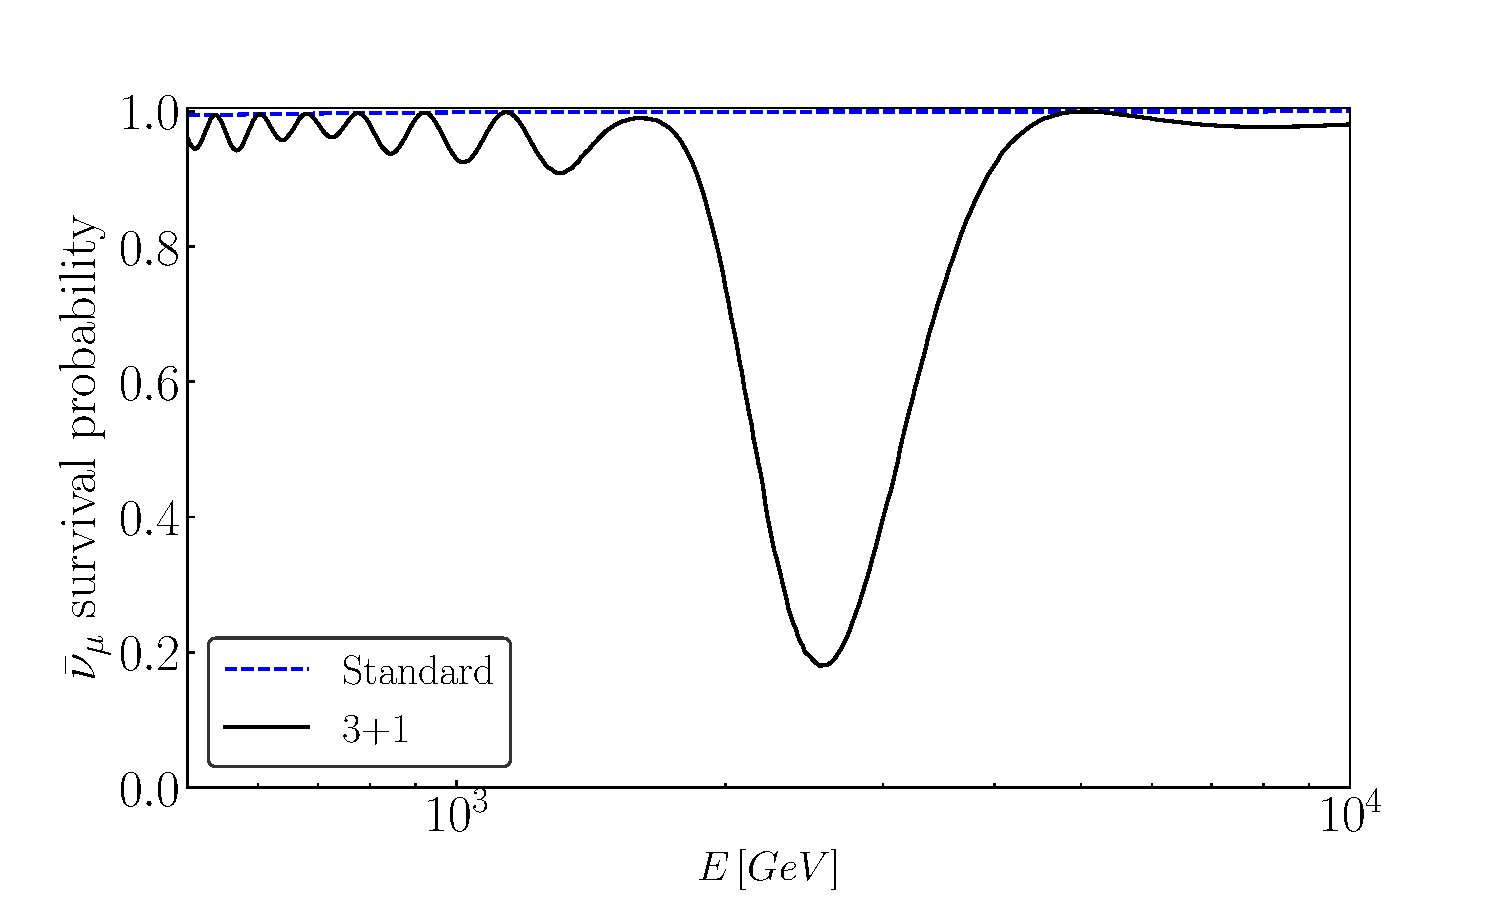
\includegraphics[width=1\linewidth]{figures/sterile_resonance.pdf}
        \caption{$\Pamam$ resonant disappearance}\label{fig:sterile_resonance}
    \end{subfigure}
    \begin{subfigure}{0.9\textwidth}
        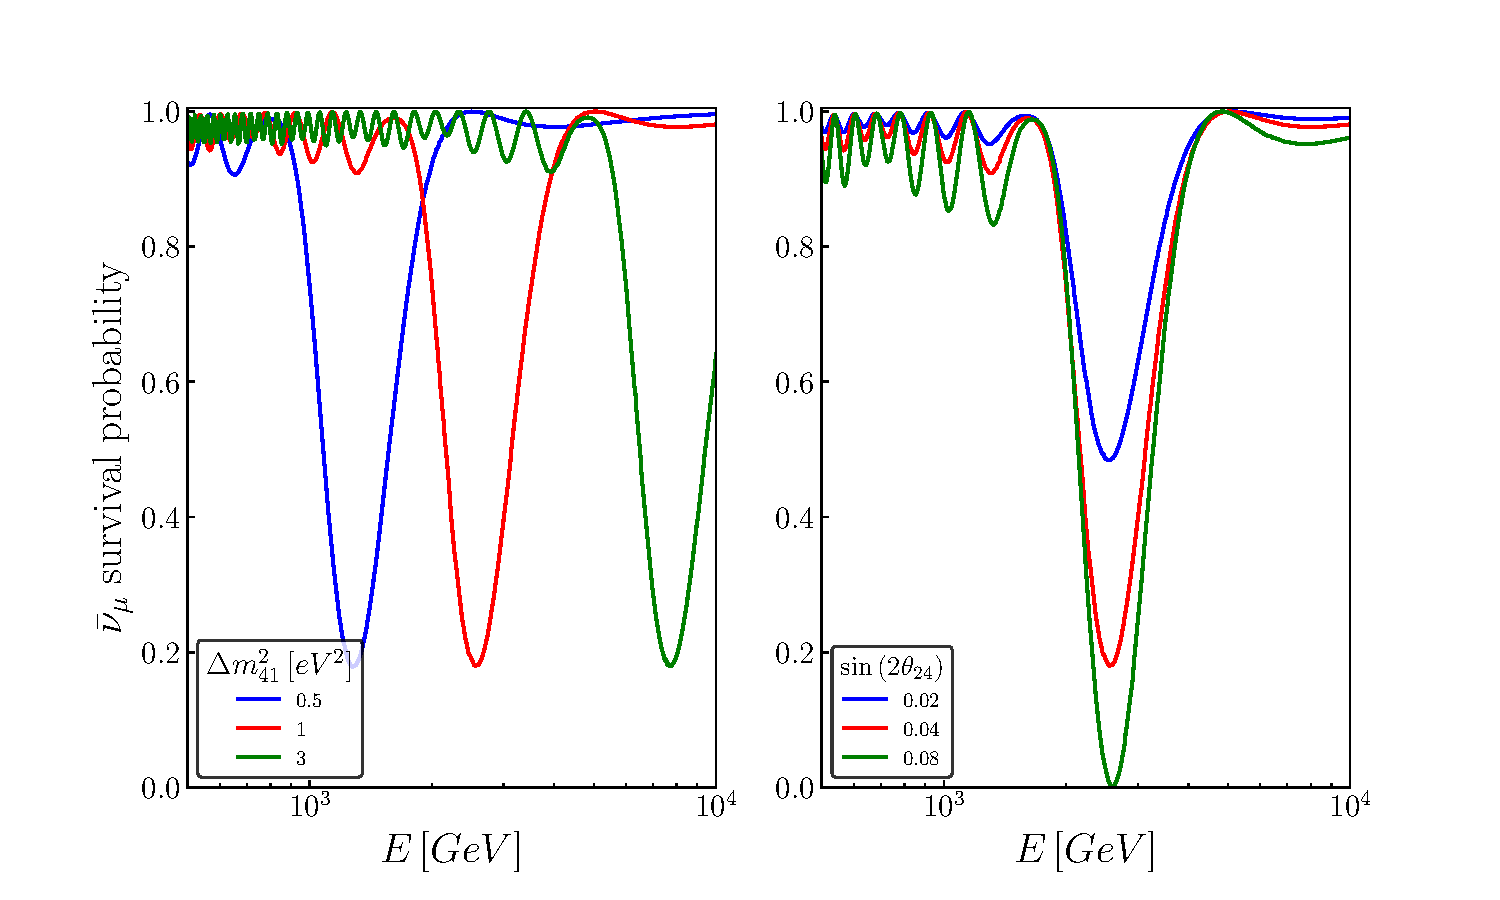
\includegraphics[width=1\linewidth]{figures/resonance_shift.pdf}
        \caption{Shifting and amplification of the resonance by altering $\dm[41]$ and $\theta_{24}$, respectively.}\label{fig:resonance_shift}
    \end{subfigure}
\end{figure}

So for a \si{\eV}-scale sterile neutrino and a non-zero $\theta_{24}$, we expect a \si{\TeV} $\anm$ disappearance.
The resonance dip is affected by the value of $\dm[41]$ and $\theta_{24}$ as shown in Fig.~\ref{fig:resonance_shift}.
We see how the value of $\dm[41]$ shifts the peak, while the mixing angle adjusts its strength. 
In the $3+0$ scenario, $\Pamam = 1$ in this range. Thus, if we are able to see a $\anm$ disappearance in the \si{\TeV} region,
we are in a good position to argue for a \si{\eV^2} scale $\dm[41]$.


%\newpage\bibliographystyle{elsarticle-num}\bibliography{ref}\end{document}